\begin{wrapfigure}{r}{6cm}
  \centering
  \vspace{-30px}
  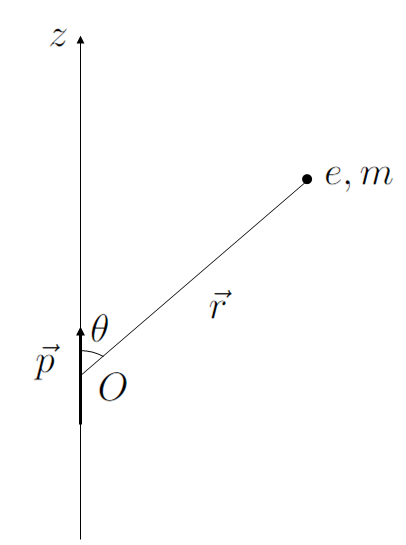
\includegraphics[width=0.25\textwidth]{images/Hinh 5.PNG}
  \begin{center}
    \figurename{ 5}
  \end{center}
\end{wrapfigure}

\vspace{-30px}
\noindent Một hạt có khối lượng $m$, điện tích $e$ chuyển động dưới tác dụng của một lưỡng cực điện được đặt cố định tại gốc toạ độ (Hình 5). Momen lưỡng cực $\vec{p}$ hướng dọc theo chiều dương của trục $Oz$. Gọi $\vec{r}(t)$ là vector vị trí của hạt tại thời điểm $t$, $\vec{r}(t)$ có độ lớn $r(t)$ và hợp với momen lưỡng cực $\vec{p}$ một góc $\theta(t)$. Biết $r(t=0)=r_{0}>0$, $\theta(t=0)=\theta_{0}$. Hằng số điện môi trong chân không là $\varepsilon_{0}$ và biểu thức của điện trường và điện thế do lưỡng cực tạo ra có dạng:
\begin{equation*}
  \vec{E}=\frac{3(\vec{p}\cdot\hat{r})\hat{r}-\vec{p}}{4\pi\varepsilon_{0}r^{3}},\quad\varphi=\frac{\vec{p}\cdot\vec{r}}{4\pi\varepsilon_{0}r^{3}}
\end{equation*}
trong đó $\hat{r}$ là vector đơn vị theo hướng $\vec{r}$.
\begin{enumerate}
  \item Giả sử hạt chuyển động trong mặt phẳng vuông góc với trục $Oz$ trên một quỹ đạo tròn quanh trục $Oz$, hãy xác định góc $\theta_{0}$ khi đó và độ lớn vận tốc $v_{0}$ của hạt.
  \item Giả sử tại $t=0$, hạt đứng yên:
        \begin{enumerate}
          \item[a.] Xác định mối liên hệ giữa độ lớn momen động lượng của hạt so với gốc toạ độ $O$ và góc $\theta$ trong quá trình chuyển động sau đó.
          \item[b.] Xác định mối liên hệ giữa độ lớn vận tốc của hạt trên phương hướng tâm $v_{r}$ và $r$ sau đó.
          \item[c.] Tìm điều kiện của $\theta_{0}$ để phạm vi chuyển động của hạt bị giới hạn, không tính đến trường hợp hạt va chạm với lưỡng cực. Trong trường hợp giá trị của $\theta_{0}$ bằng với giá trị tới hạn vừa tìm được, hãy xác định quỹ đạo chuyển động của hạt trong mặt phẳng thẳng đứng.
          \item[d.] Trong trường hợp $\theta_{0}$ không thoả mãn điều kiện tìm được ở ý trên, hãy xác định biểu thức của $r(t)$.
        \end{enumerate}
\end{enumerate}